% small.tex
\documentclass{beamer}
\usetheme{default}
\usepackage{amsmath, amsfonts, amssymb, amsthm}
\usepackage{graphicx}

\newcommand{\afe}{\frac{\alpha}{Fe}}
\newcommand{\feh}{\frac{Fe}{H}}

\newcommand{\eqn}[1]{\begin{align*}
#1
\end{align*}}
\newcommand{\eqnl}[2]{\begin{align} \label{#1}
#2
\end{align}}



\newcommand{\vect}[1]{\boldsymbol{\mathbf{#1}}}
\newcommand{\degree}[1]{${#1}^{\circ}$}
\newcommand{\highlight}{ \rowcolor{lightgrass} }
\newcommand{\script}[1]{\mathcal{#1}}
\newcommand{\bl}{\big\{}
\newcommand{\br}{\big\}}
\newcommand{\Bl}{\Big\{}
\newcommand{\Br}{\Big\}}
\newcommand{\argmax}{\operatornamewithlimits{argmax}}


\newcommand{\vz}{\vect{z}}
\newcommand{\vx}{\vect{x}}
\newcommand{\vy}{\vect{y}}
\newcommand{\vp}{\vect{\pi}}
\newcommand{\vph}{\hat{\vect{\pi}}}
\newcommand{\vpmle}{\hat{\vect{\pi}}_\text{MLE}}
\newcommand{\sumn}{\sum^n_{i=1}}
\newcommand{\summ}{\sum^m_{j=1}}
\newcommand{\summo}{\sum^{m-1}_{j=1}}
\newcommand{\sumg}{\sum^g_{j=1}}
\newcommand{\sumk}{\sum^m_{k=1}}
\newcommand{\fab}{f_j}
\newcommand{\llp}{\log L(\vp)}

\begin{document}




%%%%%%%%%%%%%%%%%%%%%
\begin{frame}{Link between curves and M theoretical distributions}
	
	(Duane will cover this part I think)
	
	
	Partition the mass and accretion time into $M$ combinations of $\mathcal{M},\mathcal{T}$ where
	
	\eqn{
		\text{Sat. stellar mass:} \hspace{3mm} \bigcup \mathcal{M}_j &= [0, 10^9] M_{\bigodot}  		\\
		\text{Accretion time:} \hspace{3mm} \bigcup \mathcal{T}_j &= [0, 14] \text{Gyr} 
	}
	\eqn{
		f_j(x,y) &= P(x,y|\text{Mass}\in \mathcal{M}_j, \text{Accretion time}\in \mathcal{T}_j)
	}

\end{frame}


%%%%%%%%%%%%%%%%%%%%%
\begin{frame}{Each observation is generated from one of these M theoretical distributions}
	
	\eqn{
		\Bigg[\feh,\afe\Bigg]_{i=1}^{N} \text{i.i.d} \sim F(x,y) = \sum^M_{j=1} \pi_j f_j(x,y)
	}	
		
	\begin{figure}
			\begin{center}
				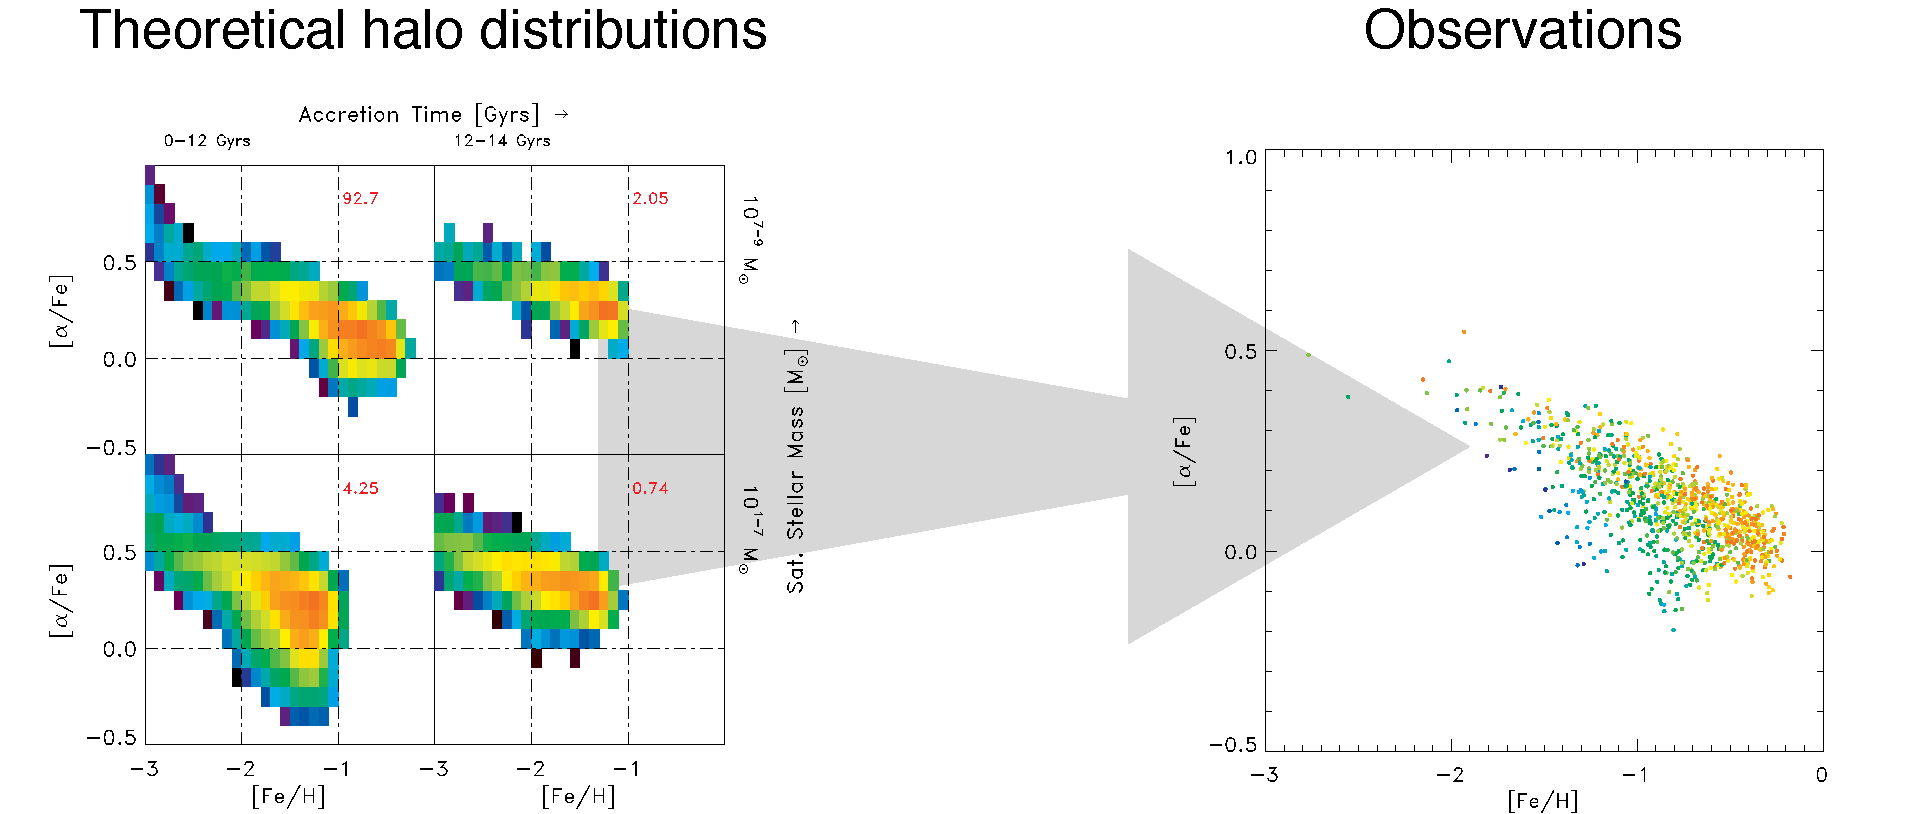
\includegraphics[width=\textwidth]{denstoobs.pdf}
			\end{center}
	\end{figure}
\end{frame}







%%%%%%%%%%%%%%%%%%%%%
\begin{frame}{Finding the mixing proportions $\vect{\pi}$}
	
	Standard maximum likelihood estimates of $\vp$ won't work
	
	\eqn{
		\log L(\vect{\pi}) &= \sumn \log \Big( \summ \pi_j \fab(x_i,y_i)  \Big)
	}
	
	
	Suppose we knew which $f_j$ each observation came from:
	
	\eqn{
		z_{ij} 	= \hspace{1mm} & 1  \hspace{4mm} \text{if} \hspace{1mm} (x_i,y_i) \sim f_j	\\
				& 0 \hspace{4mm} \text{otherwise}
	}
	
	Then
	
	\eqnl{loglike}{
		\log L(\vect{\pi}) &= \sumn \summ z_{ij}  \log \bl \pi_j  \fab(x_i,y_i) \br
	}
	
	
	
\end{frame}










%%%%%%%%%%%%%%%%%%%%%
\begin{frame}{Finding $\vph$ using expectation maximization}
	
	
	\begin{itemize}
		\item Find the expected value of the log likelihood, given the data
		\item Find the $\argmax_{\vp}$ of this expectation
		\item Repeat until $\llp$ stabilizes
	\end{itemize}
	
	
\end{frame}










%%%%%%%%%%%%%%%%%%%%%
\begin{frame}{Find the expected value of the log likelihood, given the data}
	
	
	
	\eqn{
		\text{E}_{\vp}\Big[\llp \big| \vx,\vy \Big] &= \sumn \summ \text{E}_{\vp}\big[z_{ij}|x_i,y_i\big] \bl \log \fab(x_i,y_i) + \log \pi_j  \br
	}
	\eqn{
		\hat{w}_{ij}^{(t)} 	&= \text{E}_{\vp}\Big[  z_{ij} | x_i, y_i \Big] 		\\
						&= \text{Pr}_{\vp}(z_{ij}|x_i,y_i)	\\
						&= \frac{p(x_i,y_i|z_{ij}=1)p(z_{ij}=1)}{p(x_i,y_i)}	\\
						&=  \frac{\pi_j \fab(x_i,y_i)  }{\summ \pi_j \fab(x_i,y_i)}
	}
	
	
	
\end{frame}








%%%%%%%%%%%%%%%%%%%%%
\begin{frame}{Find the $\argmax_{\vp}$ of this expectation}
	
	
	\eqn{
		\vph^{(t)} &= \argmax_{\vp} \text{E}\Big[\llp \big| \vx,\vy,\vph^{(t-1)} \Big]   
	}
	
	Accounting for the $m-1$ free parameters of $\vp$, differentiation proceeds, for $k=1,\ldots,m-1$, as:
	
	\eqn{
		\frac{\partial}{\partial \pi_k} \text{E}\Big[\llp \big| \vect{x},\vect{y}\Big]   &=      \sumn \Bl  w^{(t-1)}_{ik} \frac{1}{\pi_k} - w^{(t-1)}_{im} \frac{1}{1-\pi_1-\ldots-\pi_{m-1}}   \Br
	}
	\eqn{
		\frac{1}{\pi_k} \sumn w_{ik}^{(t-1)} &= \frac{1}{1-\pi_1-\ldots-\pi_{m-1}} \sumn w_{im}^{(t-1)}
	}
	
	Consequently
	\eqn{
		\hat{\pi}^{(t)}_k &= \frac{\sumn w^{(t-1)}_{ij}}{n}	\\
		\hat{\pi}^{(t)}_m &= 1-\pi_1-\ldots-\pi_{m-1}
	}
	
\end{frame}




%%%%%%%%%%%%%%%%%%%%%
\begin{frame}{We used a 5x5 and a 2x2 set of theoretical distributions}
		
	\begin{figure}
			\begin{center}
				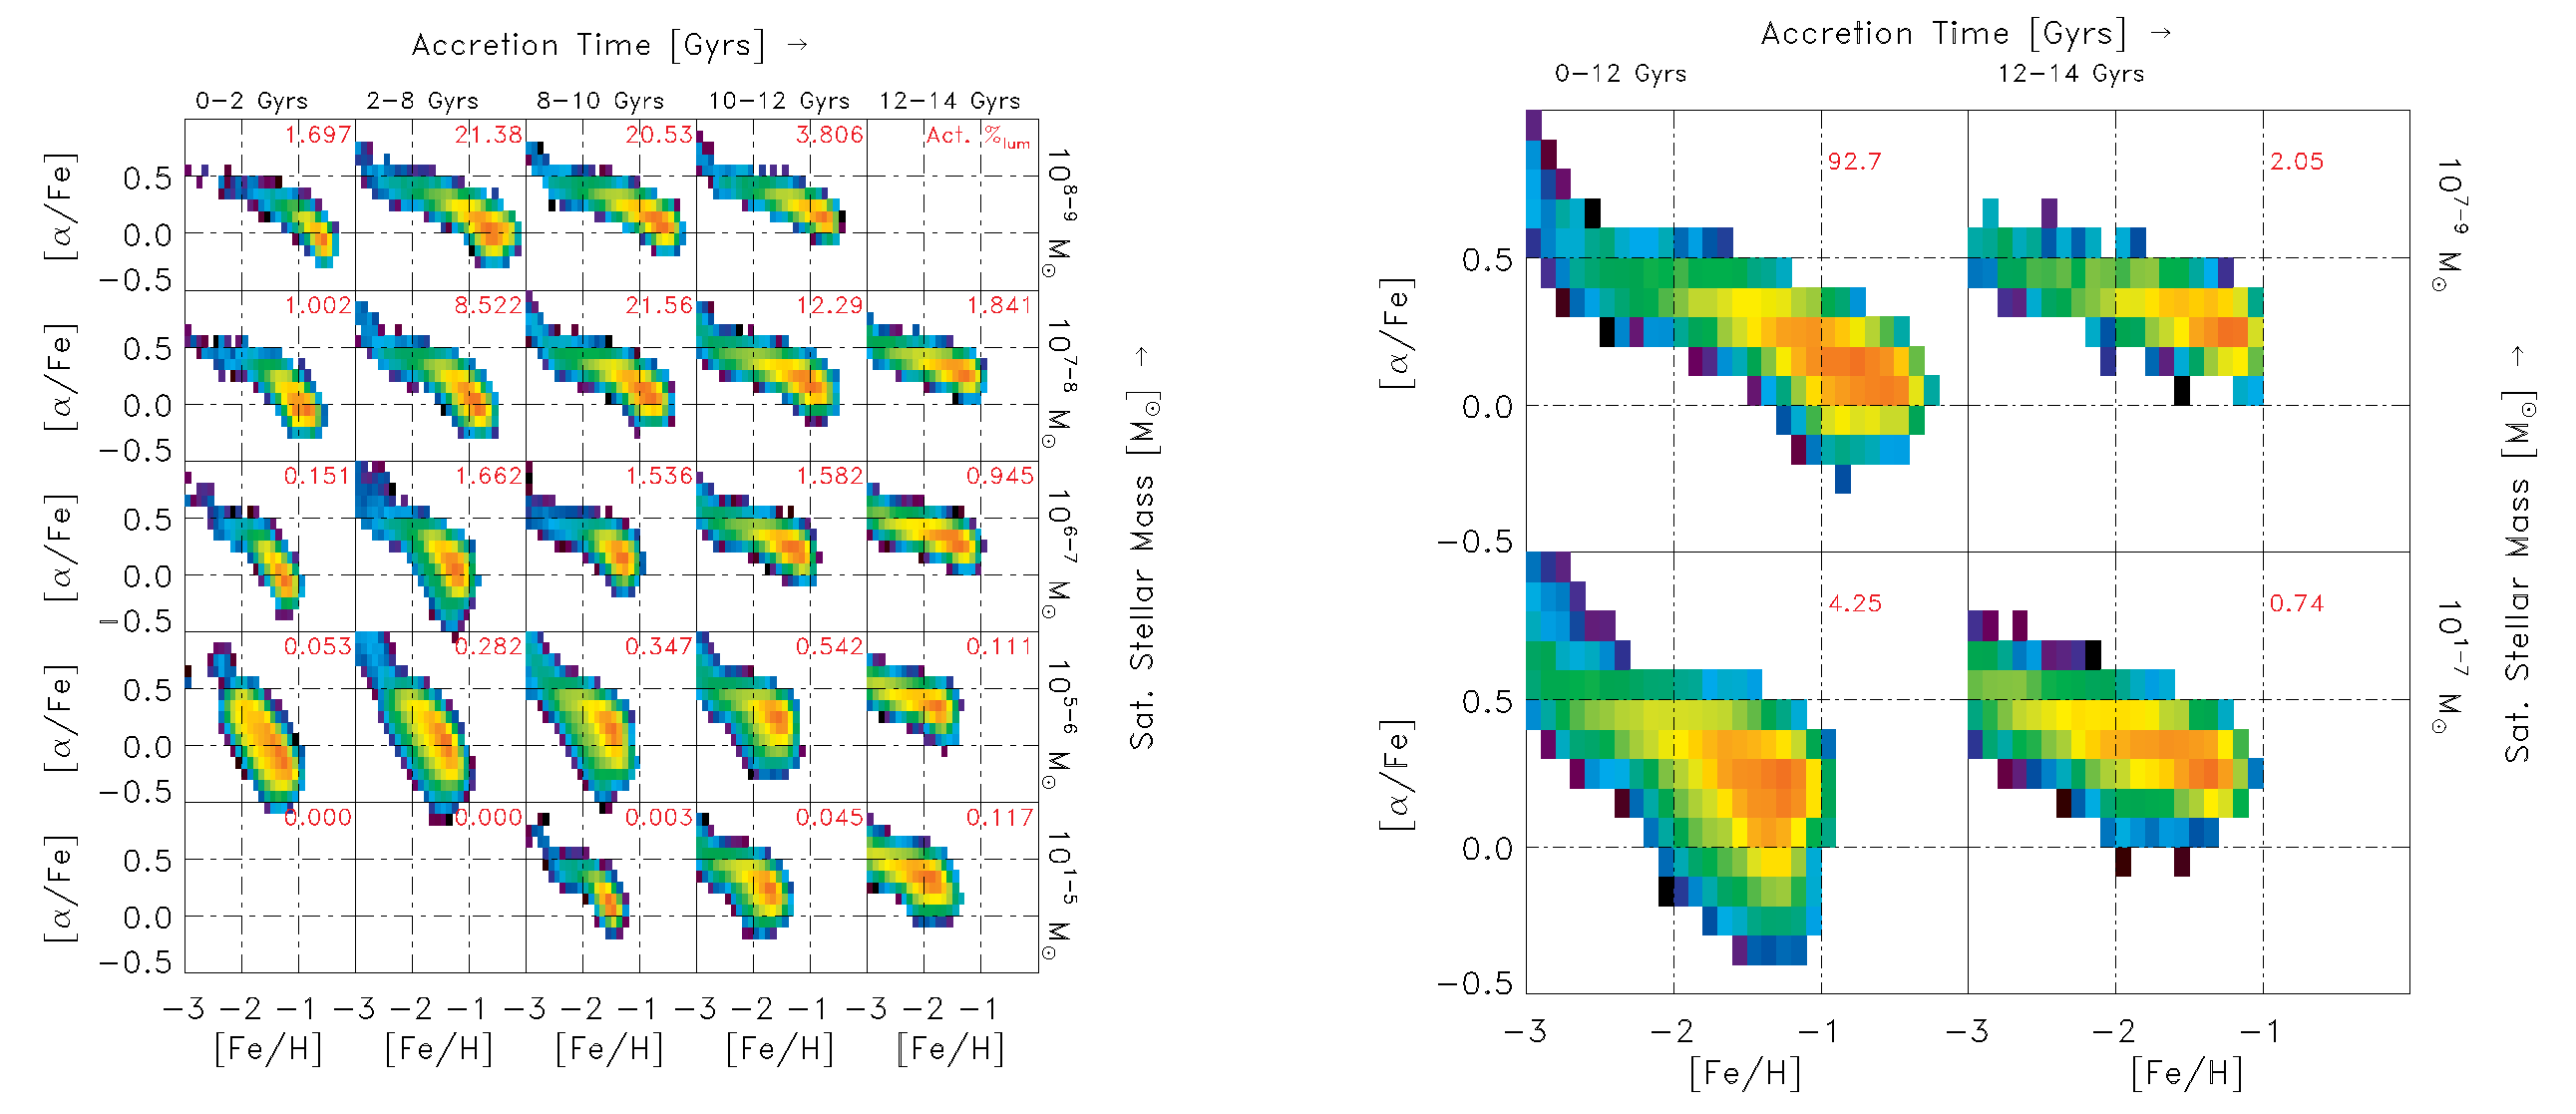
\includegraphics[width=\textwidth]{ourdens.pdf}
			\end{center}
	\end{figure}
	
	
	
	
\end{frame}











%%%%%%%%%%%%%%%%%%%%%
\begin{frame}{Simulation results}
	
	Works starting at about 1,000 observations, although larger $\vp$ values are found with smaller data sets.
	
	\begin{figure}
			\begin{center}
				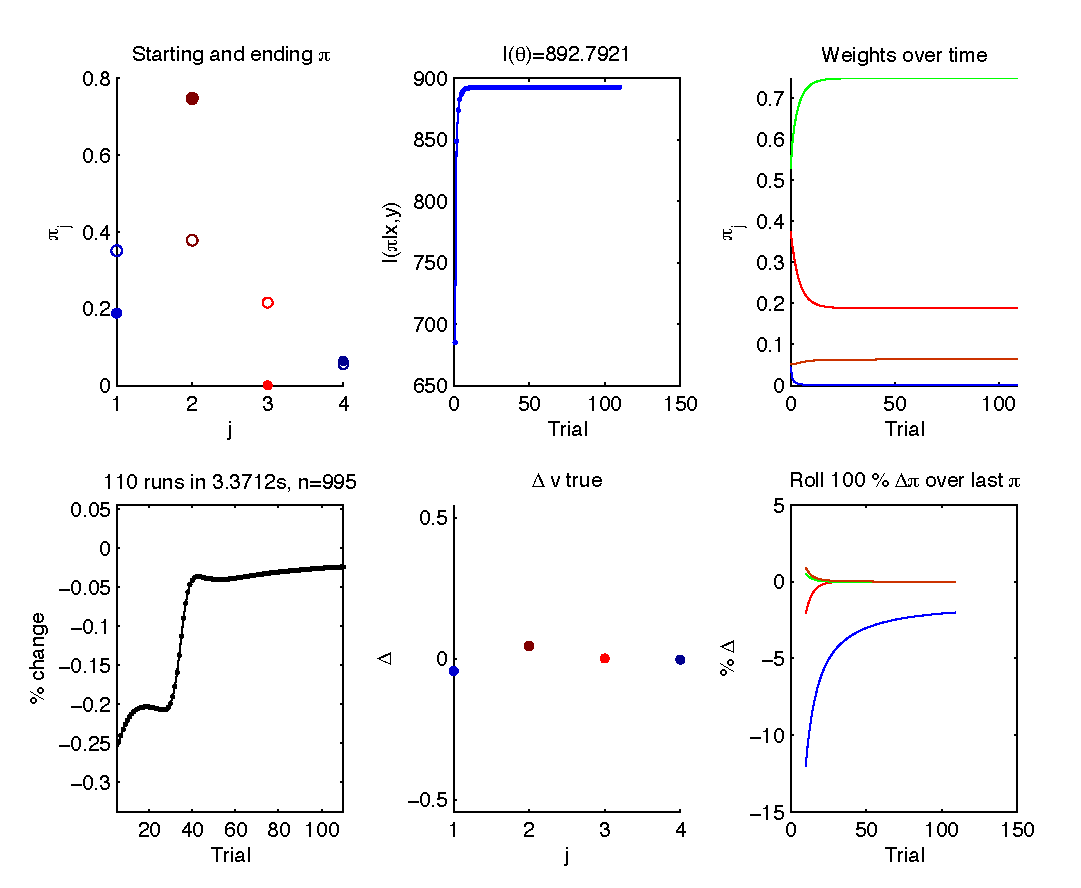
\includegraphics[scale=0.5]{diagnosticstalk.pdf}
			\end{center}
	\end{figure}
	
\end{frame}












%%%%sample
\begin{frame}{Confidence intervals}
	
	\begin{figure}
			\begin{center}
				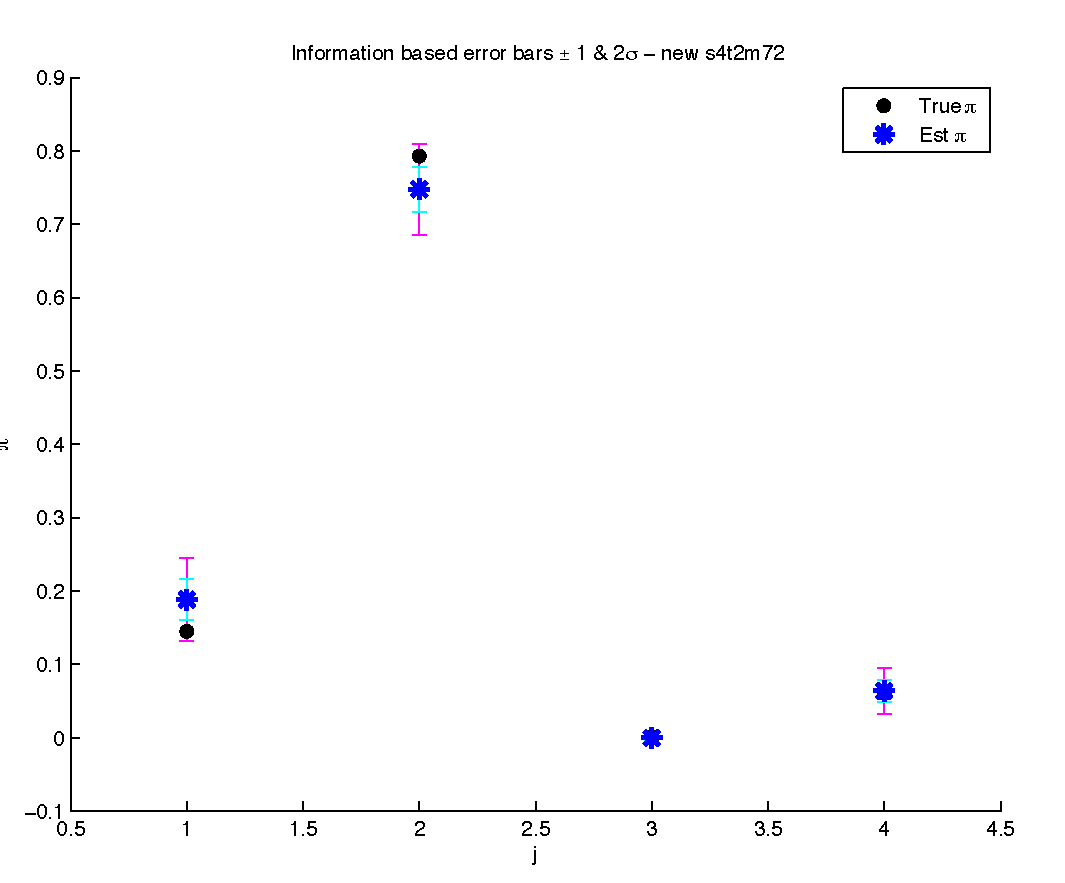
\includegraphics[scale=0.5]{errorgrid2.pdf}
			\end{center}
	\end{figure}
	
\end{frame}













%%%%sample
\begin{frame}{Correlation between $\vp$}
	
	
	
	\begin{figure}
			\begin{center}
				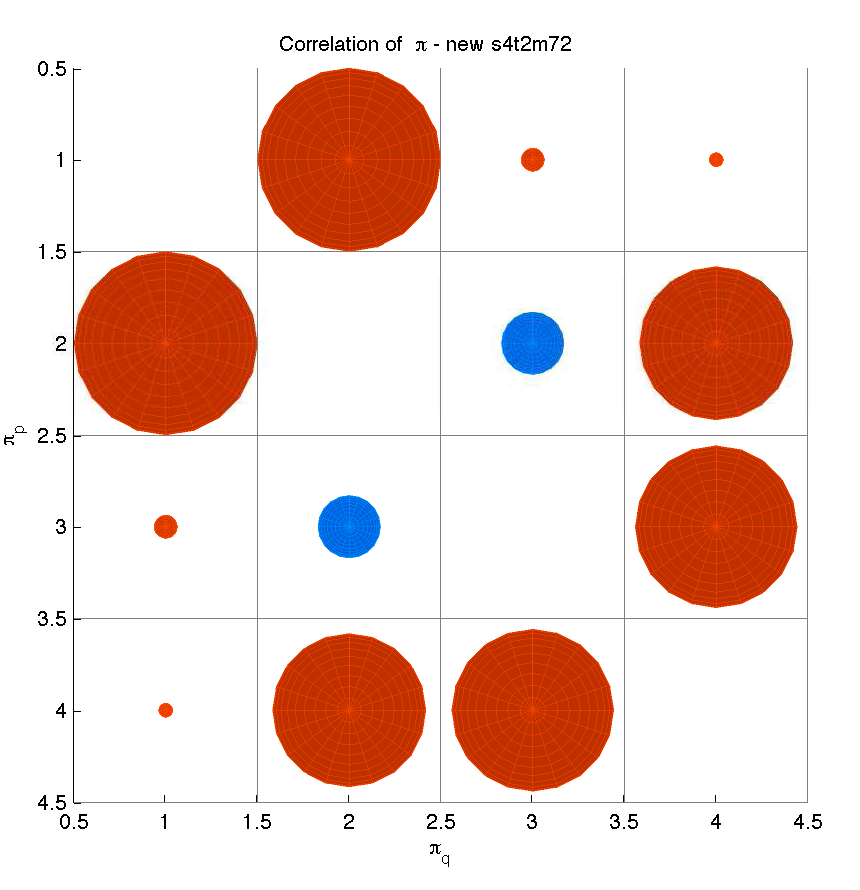
\includegraphics[scale=0.5]{correlgrid2.pdf}
			\end{center}
	\end{figure}	
	
\end{frame}








%%%%sample
\begin{frame}{Conclusion}
	
	Worked
	\begin{itemize}
		\item 2x2
		\item EM
		\item 5x5 in a few cases
		\item M-of-n bootstrapped errors
	\end{itemize}	
	
	Did not work
	\begin{itemize}
		\item 5x5
		\item Parametric bootstrapped errors
	\end{itemize}	
	
	
	Future improvements
	\begin{itemize}
		\item Non-arbitrary gridding
		\item Smoothing of $f_j$
	\end{itemize}	
	
\end{frame}



































\end{document}


